\documentclass{article}

\usepackage{fancyhdr} % Required for custom headers
%\usepackage{lastpage} % Required to determine the last page for the footer
\usepackage{extramarks} % Required for headers and footers
\usepackage[usenames,dvipsnames]{color} % Required for custom colors
\usepackage{graphicx} % Required to insert images
\usepackage{listings} % Required for insertion of code
\usepackage{courier} % Required for the courier font
\usepackage{amsmath, mathtools} %Required for math stuff
\usepackage{amssymb}
\usepackage{graphicx} % Required for including figures
\usepackage{siunitx}
\usepackage{cancel}
\usepackage{empheq}
\usepackage{tcolorbox}
\usepackage{bm}
\usepackage{float}
\usepackage{subcaption}

% Margins
\topmargin=-0.45in
\evensidemargin=0in
\oddsidemargin=0in
\textwidth=6.5in
\textheight=9.0in
\headsep=0.25in

\linespread{1.1} % Line spacing

% Set up the header and footer
\pagestyle{fancy}
\lhead{\Name} % Top left header
\chead{\Title} % Top center head
\rhead{\Date} % Top right header
\lfoot{\lastxmark} % Bottom left footer
\cfoot{} % Bottom center footer
%\rfoot{Page\ \thepage\ of\ \protect\pageref{LastPage}} % Bottom right footer
\renewcommand\headrulewidth{0.4pt} % Size of the header rule
%\renewcommand\footrulewidth{0.4pt} % Size of the footer rule

\setlength\parindent{0pt} % Removes all indentation from paragraphs

%----------------------------------------------------------------------------------------
%	NAME AND CLASS SECTION
%----------------------------------------------------------------------------------------

\newcommand{\Title}{DMDc Update} % Title of the set of notes
\newcommand{\Date}{} % Today's date
\newcommand{\Class}{} % Course/class
\newcommand{\ClassInstructor}{} % Teacher/lecturer
\newcommand{\Name}{Anthony Corso} % Your name
\newcommand{\hl}{\noindent\makebox[\linewidth]{\rule{\linewidth}{0.4pt}}}

\begin{document}

\section*{Goal}
The goal of this work is to suppress vortex shedding of a circular cylinder using model predictive control, with the model coming from Dynamic Mode Decomposition with control (DMDc) and the control coming form the rotation of the cylinder.

Broadly speaking, DMDc uses singular value decomposition to create a low-dimensional linear model for the dynamics of the system of the form
\begin{align*}
\tilde{x} &= U^T x \\
\tilde{x}_{t+1} &= A \tilde{x}_t + B u_t
\end{align*}
where the number of state variables, $x$ is much larger than the number of state variables $\tilde{x}$.

I implemented DMDc in julia at the following repository (which includes a patch for running MPC with DMDc in PyFR). Below is an update on what is working with DMDc and what is currently not working.

\section*{What works}
I've have shown that DMDc works for suppressing vortex shedding in a very narrow set of circumstances (see fig \ref{fig:dmdc_working}). Namely, when the dynamics and control matrices ($A$ and $B$) are trained from snapshots taken from the proportional control of the same system (see figure \ref{fig:training_data} for the control input of the data that $A$ and $B$ were trained from). In this case, the DMDc + MPC algorithm produces essentially the same control policy and successfully suppresses the vortex shedding.


\begin{figure}
  \centering
  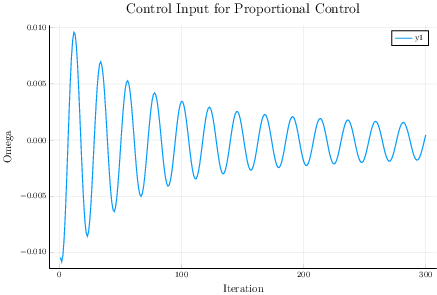
\includegraphics[scale=0.5]{../images/training_data.png}
  \caption{Control policy for the training data. The control policy comes from a proportional controller measuring the y-velocity at a point in the wake}
  \label{fig:training_data}
\end{figure}

% Figure that shows vortex shedding suppression
\begin{figure}
  \centering
  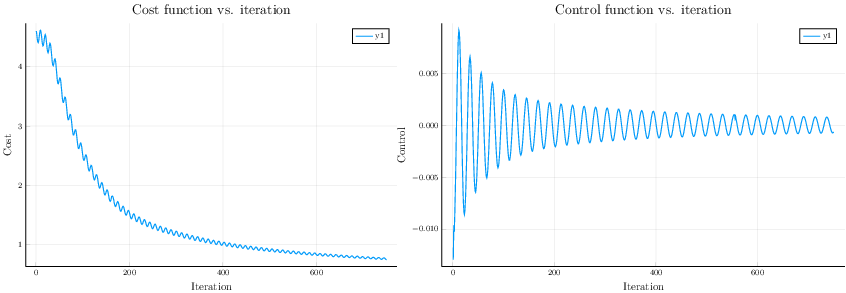
\includegraphics[scale=0.5]{../images/dmdc_working.png}
  \caption{Control policy from DMDc dynamics with MPC controller.}
  \label{fig:dmdc_working}
\end{figure}


This success, is only a modest one, however, because a working control policy was used to create the DMDc model. Unfortunately, as will be shown in the next section, the creation of a DMDc model that successfully works to suppress vortex shedding is difficult and fails in many other cases that I have tried.

\section*{What Doesn't work}

\begin{figure}
  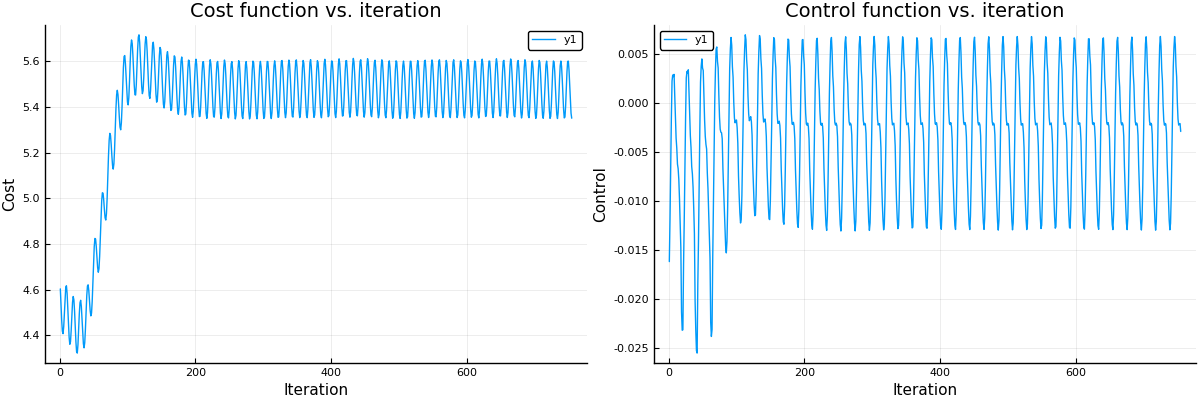
\includegraphics[scale=0.5]{../images/dmdc_offline_d1_resid_omega.png}
  \caption{Example of DMDc + MPC failing to supress vortex shedding. This failure is due to a failure in predictive capabilities of the model}
  \label{fig:failed_mpc}
\end{figure}

When $A$ and $B$ are found from training data that deviates from the proportional control data, MPC doesn't seem to work at all (see figure \ref{fig:failed_mpc} for an example). I have tracked the failure back to the fact that the predictive capabilities of DMDc seem limited to the training data that produced to the DMDc model

In order to evaluate the predictive capabilities of DMDc, I did the following:
\begin{itemize}
  \item From a sample PyFR with MPC run, I copied the dynamics matrices, $A$ and $B$, the projection matrix $U$, and all of the simulation data from the run.
  \item For each snapshot of the simulation data, I predicted the following 16 timesteps using the DMDc model. If the $t^{\rm th}$ frame of the simulation is flattened into a state vector $x_t$, and the control input is $u_t$, then we predict via
\begin{align*}
\tilde{x}_t &= U^T x_t \\
\tilde{x}^{\rm pred}_{t+1} &= A \tilde{x}_t + B u_t \\
x^{\rm pred}_{t+1} &= U \tilde{x}^{\rm pred}_{t+1}
\end{align*}

\item Then at each predicted timestep, the error in the prediction can be found via the norm $|| x^{\rm pred}_{t} - x_t ||$, where $x_t$ is the exact state, found from the simulation.

\end{itemize}

In the following examples, we show how well certain DMDc models predict the simulation dynamics of vortex suppression using proportional control. The dynamics of this process need to be accurately predicted if a similar control policy is going to be inferred with MPC.

First, consider the DMDc model that was trained on the first 300 iterations of the proportional control data (figure \ref{fig:pred_error_working}). In this case, we can see that the predicative capabilities of the model are excellent (to machine precision of exact) over the training period, and are significantly larger (although still remain small) after the training period has ended. This is the model that produced the working control policy.

Then consider a model that was trained off of the data whose control input is shown in figure ??. The predictive capability of this model on the proportional control data is order of magnitudes worse than the previous DMDc model as shown in figure \ref{fig:pred_error_not_working}. Correspondingly, this model failed to suppress vortex shedding.


% Figure that shoes the predictive power to a dmdc decomposition
\begin{figure}
  \centering
  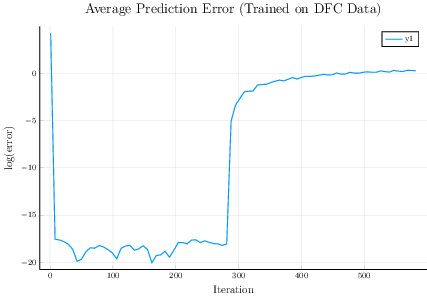
\includegraphics[scale=0.5]{../images/pred_error_working}
  \caption{The prediction error of the DMDc model trained from the proportional control data, predicting the proportional control data}
  \label{fig:pred_error_working}
\end{figure}

\begin{figure}
  \centering
  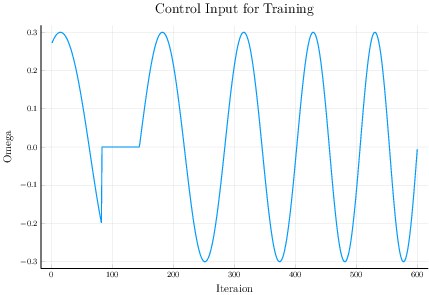
\includegraphics[scale=0.5]{../images/dfc_control_input}
  \caption{The control input for the dataset that trained the second model. The result was a model that did not accuractely predict the proportional control data.}
  \label{fig:dfc_control_input} \end{figure}
\begin{figure}
  \centering
  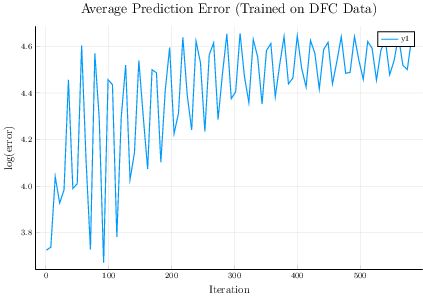
\includegraphics[scale=0.5]{../images/pred_error_not_working}
  \caption{The prediction error of the DMDc model trained from a deep flow control data set, predicting the proportional control data}
  \label{fig:pred_error_not_working}
\end{figure}

\section*{Things I've tried}

\begin{itemize}
  \item Used many different types of input training data and checked the predictive power on many other sets of data
  \item tried online computation of the $A$ and $B$ matrices, for each timestep, or every interval of 20 timesteps. Due to the sensitivy of DMDs capbility of predicting future dynamics, the constant recomputing of these matrices seems to cause the algorithm to become unstable and fail
\end{itemize}

\end{document}
